\documentclass[article]{jss}
\usepackage[utf8]{inputenc}

\providecommand{\tightlist}{%
  \setlength{\itemsep}{0pt}\setlength{\parskip}{0pt}}

\author{
Rolf Simoes, Gilberto Camara\\INPE, Brazil \And Victor Maus\\IIASA \And Alexandre Iwata\\IPEA, Brazil
}
\title{\pkg{SITS}: An R Package for Data Access, Visualisation, Filtering,
Clustering, Event Detection and Classification of Satellite Image Time
Series}

\Plainauthor{Rolf Simoes, Gilberto Camara, Victor Maus, Alexandre Iwata}
\Plaintitle{SITS: Satellite Image Time Series package}
\Shorttitle{SITS package}

\Abstract{
Using time series derived from big Earth Observation data sets is one of
the leading research trends in Land Use Science and Remote Sensing. One
of the more promising uses of satellite time series is its application
for classification of land use and land cover, since our growing demand
for natural resources has caused major environmental impacts. Given this
motivation, this package provides a set of tools for data access,
filtering, clustering and classification of satellite image time series.
}

\Keywords{satellite image time series, big Earth Observation data}

%% publication information
%% \Volume{50}
%% \Issue{9}
%% \Month{June}
%% \Year{2012}
%% \Submitdate{}
%% \Acceptdate{2012-06-04}

\Address{
      }

\usepackage{microtype} \usepackage{amsmath}

\begin{document}

\section{Introduction}\label{introduction}

Earth observation satellites provide a continuous and consistent set of
information about the Earth's land and oceans. Most space agencies have
adopted an open data policy, making unprecedented amounts of satellite
data available for research and operational use. This data deluge has
brought about a major challenge for Geoinformatics research:
\textit{How to design and build technologies that allow the Earth observation community to analyse big data sets?}

Since remote sensing satellites revisit the same place repeatedly, we
can calibrate their images so measures of the same place in different
times are comparable. These observation can be organised, so that each
measure from sensor is mapped into a three dimensional array in
space-time. From a data analysis perspective, researchers then have
access to satellite image time series (SITS). Using time series derived
from big Earth Observation data sets is one of the leading research
trends in Land Use Science and Remote Sensing.

A time-series of measurements of the same location in the surface of the
Earth can be considered as a historical record. When the images arise
for a dense record of frequent revisits, the temporal resolution of the
big data set is able to capture the most important land use changes.
Such dense time series allow researchers to which changes have taken
place in each location.

The benefits of remote sensing time series analysis arise when the
temporal resolution of the big data set is sufficient to capture the
most important changes. In this case, the temporal autocorrelation of
the data can be stronger than the spatial autocorrelation. In other
words, given data with adequate repeatability, a pixel will be more
related to its temporal neighbours rather its spatial ones. In this
case, \textit{time-first, space-later} methods will give better results
than the \textit{space-first, time-later} approach.

Time series of remote sensing data show that land cover changes do not
always occur in a progressive and gradual way, but they may also show
periods of rapid and abrupt change followed either by a quick recovery
\citep{Lambin2006}. Analyses of multiyear time series of land surface
attributes, their fine-scale spatial pattern, and their seasonal
evolution leads to a broader view of land-cover change. Satellite image
time series have already been applied to applications such as mapping
for detecting forest disturbance \citep{Kennedy2010}, ecology dynamics
\citep{Pasquarella2016}, agricultural intensification
\citep{Galford2008} and its impacts on deforestation \citep{Arvor2012}.

his work combines SITS with statistical learning. In a broad sense,
statistical learning refers to a class of algorithms for classification
and regression analysis \citep{Hastie2009}. These methods include linear
and quadratic discrimination analysis, support vector machines, random
forests and neural networks. In a typical classification problem, we
have measures that capture class attributes. Based on these measures,
referred as training data, one's task is to select a predictive model
that allows inferring classes of a larger data set.

There has been much recent interest in using classifiers such as support
vector machines \citep{Mountrakis2011} and random forests
\citep{Belgiu2016}. Most times, researchers use a
\emph{space-first, time-later} approach, where the dimension of the
decision space is limited to the number of spectral bands or their
transformations. Sometimes, the decision space is extended with temporal
attributes. To do this, researchers filter the raw data to get smoother
time series \citep{Brown2013, Kastens2017}. Then, using software such as
TIMESAT \citep{Jonsson2004}, they derive a small set of phenological
parameters from vegetation indexes, like beginning, peak, and length of
growing season \citep{Estel2015, Pelletier2016}. These approaches do not
use the power of advanced statistical learning techniques to work on
high-dimensional spaces and with big training data sets
\citep{James2013}. They have one thing in common: raw time series data
is considered too noisy to be used directly. This leads to the question:
\emph{do noise removal and homogenization steps reduce the information present in the satellite image time series?}

An alternative approach, proposed in this package, is to use the full
depth of satellite image time series to create larger dimensional
spaces. We tested different methods of extracting attributes from time
series data, including those reported by \cite{Maus2016},
\cite{Pelletier2016} and \cite{Kastens2017}. Our conclusion is that part
of the information in raw time series is lost after filtering or
statistical approximation. By choosing a statistical classifier which is
robust to noise, one should be able to get better results than current
approaches. Thus, the method we developed has a deceptive simplicity:
\emph{use all the data available in the time series samples}. The idea
is to have as many temporal attributes as possible, increasing the
dimension of the classification space. In this work, we used the MODIS
MOD13Q1 product with 23 samples per year per pixel, and 4 bands (NVDI,
EVI, nir and mir). By taking a series of labelled time series, we feed
the statistical inference model with a 92-dimensional attribute space.
Our experiments found out that modern statistical models such as support
vector machines, and random forests perform better in high-dimensional
spaces than in lower dimensional ones.

\section{Data Handling in SITS}\label{data-handling-in-sits}

The basic data unit in the sits package is the SITS tibble, which is a
way of organizing a set of time series data with associated spatial
information. In R, a ``tibble'' differs from the traditional data frame,
insofar as a tibble can contain lists embedded as column arguments.
Tibbles are consistent with the ``tidyverse'', a collection of R package
designed to work together in data manipulation. The ``tidyverse''
includes packages such as ``ggplot2'', ``dplyr'' and ``purrr''. The
``SITS'' package makes extensive use of the ``tidyverse''.

For a better explanation of how the ``SITS tibble'' works, we will read
a data set containing samples of land cover data for the state of Mato
Grosso (MT). This state has 903,357 km\textsuperscript{2} of extension,
being the third largest state of Brazil. It includes three of Brazil's
biomes: Amazonia, Cerrado and Pantanal. It is the most important
agricultural frontier of Brazil and is Brazil's largest producer of
soybeans, corn and cotton.

We used the MOD13Q1 product from NASA from 2001 to 2016, provided every
16 days at 250-meter spatial resolution in the Sinusoidal projection. To
do the analysis, we selected the Normalized Difference Vegetation Index
(NDVI) and the Enhanced Vegetation Index (EVI), and the original near
infrared (NIR) and middle infrared (MIR) bands. We defined nine classes:
(1) forest, (2) cerrado, (3) pasture, (4) soybean-fallow (single
cropping), (5) fallow-cotton (single cropping), (6) soybean-cotton
(double cropping), (7) soybean-corn (double cropping), (8)
soybean-millet (double cropping), (9) soybean-sunflower (double
cropping). According to the Brazilian Institute of Geography and
Statistics (IBGE), crop classes (4)-(9) accounted for more than 93\% of
MT agricultural land area in 2015. Crop and pasture ground data was
collected by researchers Alexandre Coutinho, Julio Esquerdo and Joao
Antunes from the Brazilian Agricultural Research Agency through farmer
interviews in October 2009 and in October 2013. Samples for cerrado and
forest classes were provided by Rodrigo Bergotti. Ground samples for
soybean-fallow class were provided by Damien Arvor, based on his
previous work \citep{Arvor2012}.

\begin{CodeChunk}

\begin{CodeInput}
> # retrieve a set of samples from an RDS file
> embrapa_mt.tb <- readRDS(system.file("extdata/time_series/embrapa_mt.rds", package = "sits"))
> embrapa_mt.tb
\end{CodeInput}

\begin{CodeOutput}
# A tibble: 2,115 x 7
   longitude latitude start_date   end_date   label    coverage
       <dbl>    <dbl>     <date>     <date>   <chr>       <chr>
 1  -55.1852 -10.8378 2013-09-14 2014-08-29 Pasture mod13q1_512
 2  -57.7940  -9.7573 2006-09-14 2007-08-29 Pasture mod13q1_512
 3  -51.9412 -13.4198 2014-09-14 2015-08-29 Pasture mod13q1_512
 4  -55.9643 -10.0621 2005-09-14 2006-08-29 Pasture mod13q1_512
 5  -54.5540 -10.3749 2013-09-14 2014-08-29 Pasture mod13q1_512
 6  -52.4572 -10.9512 2013-09-14 2014-08-29 Pasture mod13q1_512
 7  -52.1443 -13.9981 2013-09-14 2014-08-29 Pasture mod13q1_512
 8  -57.6907 -13.3382 2015-09-14 2016-08-28 Pasture mod13q1_512
 9  -54.7034 -16.4265 2015-09-14 2016-08-28 Pasture mod13q1_512
10  -53.6543 -15.7155 2014-09-14 2015-08-29 Pasture mod13q1_512
# ... with 2,105 more rows, and 1 more variables: time_series <list>
\end{CodeOutput}
\end{CodeChunk}

this needs to be explained further\ldots{}.

\section{Using the Web Time Series Service
WTSS}\label{using-the-web-time-series-service-wtss}

To get a remote sensing time series, one first organises a large set of
EO data as a 3D array. From each pixel location in the array, one can
extract a time series of one or more variables for a temporal interval.
The WTSS service is independent of the actual data architecture used for
3D array store. It can work with solutions such as flat files, MapReduce
distributed datasets, array databases or object-relational databases. We
have implemented the service using both a set of flat files and the
SciDB array database management system \citep{Stonebraker2013}, with the
same external interface.

\begin{CodeChunk}

\begin{CodeInput}
> URL <- "http://www.dpi.inpe.br/tws/wtss"
> wtss_inpe <- sits_infoWTSS(URL)
\end{CodeInput}

\begin{CodeOutput}
-----------------------------------------------------------
The WTSS server URL is http://www.dpi.inpe.br/tws/wtss
Available coverages: 
itobi
merge
mixl8mod
mixl8mod_f
mod13q1_512
------------------------------------------------------------
\end{CodeOutput}
\end{CodeChunk}

\begin{CodeChunk}

\begin{CodeInput}
> # get information about a specific coverage
> sits_coverageWTSS(URL,"mod13q1_512")
\end{CodeInput}

\begin{CodeOutput}
----------------------------------------------------------------------------------
Coverage: mod13q1_512
Description: Vegetation Indices 16-Day L3 Global 250m
Source: https://lpdaac.usgs.gov/dataset_discovery/modis/modis_products_table/mod13q1
Bands: 
  name                            description
1 ndvi                      250m 16 days NDVI
2  evi                       250m 16 days EVI
3  red  250m 16 days red reflectance (Band 1)
4  nir  250m 16 days NIR reflectance (Band 2)
5 blue 250m 16 days blue reflectance (Band 3)
6  mir  250m 16 days MIR reflectance (Band 7)

Spatial extent: (-180, -90) - (180, 90)
Spatial resolution: (0.00208334, 0.00208334)
Projection CRS: +proj=longlat +ellps=WGS84 +datum=WGS84 +no_defs
Time range: 2000-02-18 to 2017-02-18
Temporal resolution: 16 days 
----------------------------------------------------------------------------------
\end{CodeOutput}

\begin{CodeOutput}
# A tibble: 1 x 13
    wtss.obj        name            bands start_date   end_date
      <list>       <chr>           <list>     <date>     <date>
1 <S4: WTSS> mod13q1_512 <tibble [6 x 4]> 2000-02-18 2017-02-18
# ... with 8 more variables: timeline <list>, xmin <dbl>, xmax <dbl>,
#   ymin <dbl>, ymax <dbl>, xres <dbl>, yres <dbl>, crs <chr>
\end{CodeOutput}

\begin{CodeInput}
> # choose a coverage
> coverage <- "mod13q1_512"
> # recover all bands
> bands <- c("ndvi", "evi", "nir")
> # a point in the transition forest pasture in Northern MT
> long <- -55.57320
> lat <- -11.50566
> # obtain a time series from the WTSS server for this point
> series.tb <- sits_getdata(longitude = long, latitude = lat, URL = URL, coverage = "mod13q1_512", bands = bands)
> # plot the series
> sits_plot (series.tb)
\end{CodeInput}


\begin{center}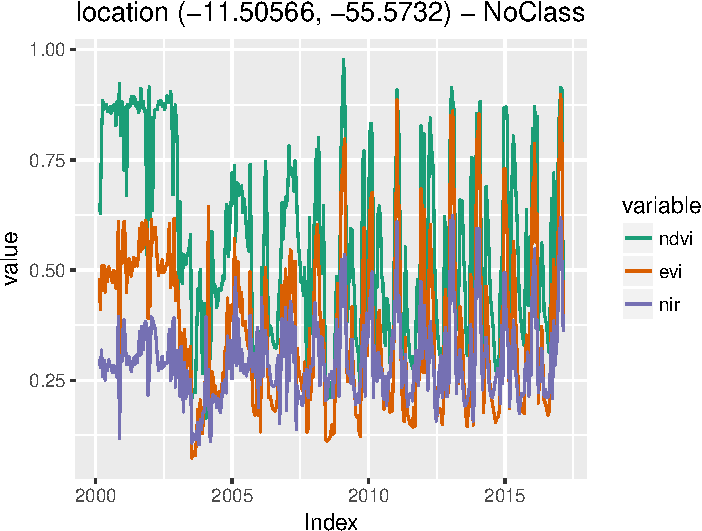
\includegraphics{sits_files/figure-latex/unnamed-chunk-7-1} \end{center}

\end{CodeChunk}

\section*{Acknowledgments}

This work is supported by the São Paulo State Foundation (FAPESP) under
grant 2014/08398-6 (``e-sensing: Big Earth observation data analytics
for land use and land cover change information''), and by the Germany
International Klimate Initiative under the RESTORE+
grant17\_III\_084\_Global\_A\_RESTORE+ (``RESTORE+: Addressing Landscape
Restoration on Degraded Land in Indonesia and Brazil''). Gilberto
Camara's work is also supported by CNPq (grant 312151/2014-4).

\bibliography{e-sensing.bib}


\end{document}

